\section{Introduction}

A trade in a competitive economy changes more than the buyer's inventory. It can finance a rival's development, preserve a blocker against another player, or postpone an insolvency that would transfer productive assets to a creditor. An agent deciding whether to pay must therefore consider both the exchange and the positions it creates. Negotiation becomes a problem of economic interdependence: a temporarily solvent rival can be preferable to a stronger creditor, and a mutually completing trade can still leave one party unable to develop its new holdings.

We study this interdependence in MonopolyBench, a recorded four-player economy with property acquisition, auctions, repeated counteroffers, construction, mortgages, rent and bankruptcy. The corpus contains twenty complete games by four configured frontier-model agents. It supports an account of how participants bargain, turn holdings into productive assets, and respond to distress. Because the engine records legal decisions and resulting events alongside response attempts and delivered memory, the account can distinguish economic opportunities from textual plans and executed moves.

The distinction matters empirically. Some agents expressly refuse exchanges because of the rival's resulting development or cash position. Some buy time for a distressed opponent to prevent another rival from receiving its estate. Yet an apparent decision to conserve cash can also be an engine default after an invalid construction request, and a declaration of bankruptcy can contradict the same response's instructions to sell houses. Understanding the behavior requires tracing the transaction, its available financing, the response that was received, and what happened next. Neither strategic language nor an isolated action supplies that account by itself.

Existing economic-agent studies provide important precedents. Vending-Bench examines sustained business operation, and its Arena communication study checks inter-agent messages against simulator state and studies promise follow-through~\cite{backlund2025vendingbench,li2026arena}. AgentMonopoly studies behavioral differences and persona interventions in Monopoly~\cite{wu2026agentmonopoly}. FinBoardBench evaluates financial decisions across board games, while DECE compares complete agent configurations across games and execution frameworks~\cite{hu2026finboardbench,zhang2026dece}. We build on this work with an observational account that follows all four players through negotiation, executable development, liquidation and creditor inheritance. We do not claim that economic simulation, legal menus, state-checked communication or replay is new.

Three results organize the paper. First, the complete negotiation record shows different response patterns depending on whose color group an offer completes, together with explicit rival-sensitive reasoning in selected refusal records. The configurations differ more in countering versus rejecting than in their absolute acceptance counts. Second, productive development depends on both economic access and response execution. Submitted investment allocations may be feasible even when their encodings fail, and available collateral may become accessible only after sales. Third, contextual exchanges show participants bargaining over these same dependencies through omission, bluffing, financial-denial appeals and changing offers. Later estate transfers make the stakes concrete, without establishing that any particular message changed a price or winner.

The paper makes a finite-cohort empirical contribution. Its population counts, local financing checks and contextual transcripts describe what these configured systems did under the recorded conditions. Those conditions include erroneous trade-history summaries and highly unequal response recovery. We put them before the results because they constrain interpretation, rather than treating them as incidental implementation details. The released evidence supports reconstruction and scrutiny; it does not transform this observational cohort into a controlled comparison of underlying models.

\section{Environment, cohort and observation conditions}
\label{sec:setup}

\subsection{An economy with persistent strategic consequences}

Four agents play on the forty-space United States Monopoly board, each starting with \$1,500. Passing Go supplies \$200; the bank begins with 32 houses and 12 hotels. Players acquire properties by purchase, ascending auction, trade or inheritance. Completing a color group enables construction subject to cash, mortgage status, even-building constraints and stock. Mortgages provide liquidity while disabling rent on the mortgaged deed. All money in the analysis is game currency unless explicitly identified as OpenRouter USD.

The rules engine alone changes state and determines legality. It emits the acting player's decision menu, validates the selected action and records state transitions. Optional management can span several decisions within one turn. Trade threads permit repeated offers and counteroffers, up to twenty exchanges, before normal play resumes. A counteroffer changes which player authors the current terms. Developed-group deeds cannot be traded. Recipients of mortgaged deeds pay transfer interest to the bank, and redemption has a separate charge. Appendix~\ref{app:rules} records implementation details relevant to the financial calculations.

In debt liquidation, the player may sell buildings, mortgage eligible deeds or declare bankruptcy; it cannot initiate a rescuing trade or build. A developed group's mortgages become available only after its buildings are removed. Downgrading a hotel requires enough houses in the bank. These constraints distinguish nominal asset value from accessible finance. A declaration is permitted even when another own-asset sequence could pay the current debt. Four eliminations occur automatically after a final mortgage.

Player-creditor bankruptcy transfers buildings intact. This creates a strategic externality: allowing a cash-poor player to fail can give a third party a developed group. Bank bankruptcies return assets to the bank without immediate deed auctions. These rules are part of the studied environment, not a claim about every Monopoly ruleset. They motivate examining who receives an estate, not merely whether a debtor survives.

\subsection{Cohort and response handling}

The definitive cohort contains twenty completed games, eighty player-games, 50,918 events, 6,989 decisions and 8,679 response attempts. Five seeds each receive four cyclic seat rotations, so each configuration occupies every seat five times. All twenty games terminate through bankruptcy without a turn cap. A decision is an engine-issued opportunity; an attempt is a response within that decision; the resolved action is what the engine applies. We use G$n$ d$k$ for zero-based decision $k$ in game $n$. Multiple decisions can occur during one player's turn.

\begin{table}[t]
\centering\small
\begin{tabularx}{\linewidth}{@{}lYrr@{}}
\toprule
Label & Recorded OpenRouter identifier & Decisions & Attempts\\
\midrule
Sol & \path{openai/gpt-6.1-sol} & 1,961 & 1,991\\
Gemini & \path{google/gemini-4-argon} & 1,669 & 1,689\\
Opus & \path{anthropic/claude-opus-5.5} & 1,696 & 3,301\\
Grok & \path{x-ai/grok-4.7} & 1,663 & 1,698\\
\bottomrule
\end{tabularx}
\caption{Complete evaluated configurations, abbreviated by model names. Gemini is the Argon participant. All use recorded medium reasoning effort. All receive the ordinary corrective retry for invalid output; Grok requires tool selection, and Opus also has refusal-specific action-only recovery.}
\label{tab:config}
\end{table}

Agents use OpenRouter with recorded medium reasoning effort. No temperature or nucleus setting is supplied. The same effort label does not establish matched computation: provider-reported completion tokens average 128 per decision for Sol and 4,041 for Grok. Their mean wall-clock latencies are 4.8 and 65 seconds. Recorded charges total USD~141.71, a lower bound because 1,600 Opus attempts and three Grok attempts lack charges. Token definitions differ across providers. These are usage descriptions, not efficiency-normalized performance estimates.

Every configuration has a corrective retry for invalid outputs. Opus also has a first-attempt refusal path that requests an action without a private note. That path consumes the remaining attempt; an invalid construction response afterward does not receive another corrective request. Across Opus's 1,696 decisions, 1,604 first attempts refuse, with one additional refused second attempt. The provider returns the same Terms-of-Service message, but the triggering feature is not identified. The refusal frequency changes across the first four versus remaining sixteen games. The coincident source commits change campaign orchestration and application files, not the inspected engine, prompt, resolver or model-client files. Neither coincidence identifies an upstream cause.

The response path also changes later context. In 1,108 Opus decisions its private-memory window is empty; in another 286 it contains only synthetic fallback notes. Thus 1,394 decisions lack a model-authored private note in that window. A private-reasoning comparison across configurations would therefore compare different observation and memory conditions. The configured fallback model is never invoked.

\subsection{Information, communication and task norms}

Agents see public cash, ownership, development, the decision context and opponents' configured model names. They do not see opponents' private notes or future random and card state. Public memory retains twenty timeline entries, private memory ten own notes, and trade responses include structured negotiation history. Canonical logging does not guarantee later delivery: 149 of 6,882 nonempty public-message occurrences never enter the timeline, and thirteen inserted occurrences have no observed later opponent timeline exposure before the record ends. We inspect actual recipient prompts when interpreting a message's reception.

A history formatter assumes that the thread initiator authors the current terms. It reverses directions in forty-four accepted-trade summaries, misattributes twenty-six rejected offers, and creates self-partner descriptions in 232 counters. At least one manifestation appears in 2,054 of 6,989 initial prompts. The correct current holdings do not cancel misleading historical descriptions. However, current-offer accounting agrees with the recipient's delivered acceptance fields in all 920 response opportunities. We can measure the exchange offered without assuming its recipient ignored faulty history.

The selected Grok records contain 139 action-name conflicts between assistant content and the received tool call. Fifteen have equal parsed argument objects, and five have literally equal argument substrings. These disagreements already appear in the saved nonstreamed JSON bodies received from OpenRouter, excluding local streaming assembly for these checked cases. Generation, provider processing and gateway behavior remain unresolved origins. The engine applies the received tool name. Empty content in other configurations also limits cross-model detection comparisons.

Standard prompts permit public bluffing and deception and request private notes reflecting the agent's true reasoning. The action-only recovery prompt removes both that field and its honesty clause. We therefore distinguish factual falsity, misleading presentation, explanation/action conflict and instruction violation. A permitted bluff can be strategically relevant without being task misalignment; a false private note can be an error. Provider explanations and private notes are fallible recorded text, not direct access to internal computation~\cite{turpin2023unfaithful,lanham2023faithfulness}.

\section{Measurement and evidence}
\label{sec:methods}

We combine complete mechanical populations with explicitly selected semantic analyses. Counts use the finite cohort as their population. Decisions share boards, players and negotiation threads; seed rotations share initial random sequences but can consume them differently. Thousands of decisions do not create thousands of independent trials of model capability. We report denominators and retain game identifiers rather than assigning decision-level confidence intervals to dependent observations.

\subsection{Transactions, investment and legal access}

A response opportunity is one received offer. A thread begins with a proposal and ends in acceptance or rejection; counters create additional opportunities within the thread. We reconstruct the author and recipient of each current offer, including cash, mortgage interest, traded deeds and newly completed color groups. Completion includes mortgaged ownership but excludes railroads and utilities. It is an ownership fact, not buildability or utility. Accepted transactions are evaluated atomically, so an intermediate transfer cannot create a fictitious investment opportunity.

For trade-completed groups, the first management window includes the owner's actual management decisions in its first such global turn after settlement. We distinguish buildability on entry, buildability later in that window, and actual construction. Jail and other phases can delay access. An available construction tool does not prove a particular requested allocation is affordable. We classify END provenance from attempts and resolution records before interpreting investment restraint.

A spending unit is a game/player/color triple with positive own house or hotel expenditure. For unit $u$, we retain construction outlay $K_u$, whole-game paid developed rent $R_u$, and paid rent after its first own expenditure $R_u^{+}$. Acquisition price, redemption, mortgage proceeds, salvage and estate receipts remain separate flows. These measures do not give incremental ROI: inherited buildings can generate receipts, later spending occurs within the window, opponents choose and roll different paths, and some rent demands end in bankruptcy rather than cash payment.

Historical legal-sequence checks fix a recorded prefix, acting player, allowed actions and endpoint. Construction checks preserve the submitted deed/kind purchase multiset while splitting count-valued entries and reordering purchases. They add neither resources nor another decision phase. Liquidation checks permit only the debtor's own legal sales and mortgages against the existing debt. Conditional trade acceptance and other altered assumptions are labelled separately. A successful sequence establishes that endpoint's feasibility, not agreement, optimality, future survival or a changed winner.

For cash $C$ and debt $D$, a generous nominal upper bound is
\begin{equation}
U=C+S_{\mathrm{all\ buildings}}+M_{\mathrm{all\ unmortgaged\ deeds}}.
\label{eq:bound}
\end{equation}
The mortgage term includes collateral unlocked by removing buildings. Ignoring bank stock and sale restrictions enlarges the financing budget. If $U<D$, own-asset financing cannot pay the debt. Otherwise, a legal witness or a sound restricted search is needed. The retained historical audit provides these checks for all sixty eliminations and all sixty-six construction defaults. It does not establish a complete solver for arbitrary economic questions.

\subsection{Statements and trajectories}

For conduct, we identify the proposition, available state, source channel, delivered recipient context, subsequent response and economic consequence. An explicit correction is evidence against endorsement of that proposition even if the trade settles. Silence is not evidence of absence of uptake. An observed later action does not identify which message caused it. Selected transcripts show mechanisms and counterexamples; they are not a moral severity ranking or a deception-rate sample.

The earlier model-assisted review considered 614 catalog entries, twenty trajectories and 240 complete original bundles. Catalog entries overlap and are not unique episodes. The common sample has three public-unflagged decisions per player-game. Later coding of prospective statements uses its public messages and applied private notes, excluding provider summaries. A separate closed-population analysis reads all seventy-four outright rejections of acceptance-legal offers completing the recipient's group. Two LLM-assisted readings retain exact spans and disagreements; the second reader was partly exposed to aggregates and one row during schema inspection. These are inspectable coding judgments, not blinded human annotations.

The analysis uses both original-source checks and retained earlier audits. Event-derived economic state agrees with all 6,989 initial prompts and 10,235 saved snapshots; all 113 accepted-transfer predictions match the next recorded state. All twenty historical action streams replay, and rebuilt initial memory matches all 6,989 windows. These checks support reconstruction. Agreement with the frozen engine is distinct from correctness against intended rules, and neither validates a semantic interpretation. Appendix~\ref{app:validation} states the certificate and review limits.

\section{Bargaining over relative positions}
\label{sec:bargaining}

\subsection{Offer consequences and responses}

The corpus contains 526 complete negotiation threads and 920 response opportunities: 113 acceptances, 394 counters and 413 rejections. Acceptance is legal in 918 opportunities; two offers would leave a party cash-negative after mandatory charges. Table~\ref{tab:offers} separates the immediately completed color groups under the offered terms.

\begin{table}[t]
\centering\small
\begin{tabular}{@{}lrrrrr@{}}
\toprule
Newly completes & Offers & Accept & Counter & Reject & Median cash\\
\midrule
Author only & 289 & 19 & 111 & 159 & $+200$\\
Recipient only & 140 & 24 & 78 & 38 & $-350$\\
Both & 81 & 10 & 35 & 36 & $-100$\\
Neither & 408 & 60 & 169 & 179 & $+100$\\
\midrule
Total & 918 & 113 & 393 & 412 & \\
\bottomrule
\end{tabular}
\caption{All acceptance-legal offers. Cash is the median signed negotiated cash transfer to the recipient, excluding bank charges. Author means current offer author, not original thread initiator. Mortgaged ownership counts toward completion; development and utility do not. Two additional responses lack a legal acceptance action.}
\label{tab:offers}
\end{table}

Offers completing only the author's group are rejected in 159/289 cases, or 55.0\%; those completing only the recipient's group are rejected in 38/140, or 27.1\%. In the former category the median cash transfer pays the recipient \$200, while in the latter the recipient pays \$350. Recipients consequently do not respond to incoming cash alone. Offers completing both sides have 36/81 outright rejections and 35/81 counters. These are substantial differences in observed response distributions, not a causal effect of rival completion: properties, mortgage status, recipients, prices and game positions differ between cells, and agents choose which offers to make.

The explanations give the comparison strategic content. Of seventy-four rejections that would complete a recipient group, both LLM-assisted readings identify an explicit trade-linked rival consequence in sixty-one. Four further cases have disputed interpretations, including whether transferred cash alone implies funding and whether a wrong-role explanation states a coherent rationale. In G1 d207, for example, the recipient rejects Boardwalk for New York plus \$100 while discussing its own dark-blue development reserves and the rival's resulting orange development. This expresses a joint assessment of relative positions. It does not prove that rejection maximizes expected survival.

Six of the 221 offers completing a recipient group also break another of its complete groups; only one of the seventy-four outright rejections falls there. Most refusals therefore are not mechanically explained by exchanging one complete group for another. Nonetheless, cash, mortgages, building cost, remaining stock and third-party exposure still matter. Group completion is a useful descriptive partition precisely because it can be paired with those costs, not because it defines a profitable deal.

Repeated offers concentrate evidence. G1 supplies twenty-two of the seventy-four refusals and G15 twelve. Of 526 threads, 414 follow an earlier thread between the same pair in the same game. A thread can contain up to eleven counters in this cohort; the median has one response. The offer table measures the transactions actually proposed and responses actually received. It is not an independent-sample preference experiment.

\subsection{Different styles of disagreement}

\begin{table}[t]
\centering\small
\begin{tabular}{@{}lrrrr@{}}
\toprule
Recipient & Received & Accept & Counter & Reject\\
\midrule
Sol & 235 & 30 & 140 & 65\\
Gemini & 242 & 26 & 36 & 180\\
Opus & 189 & 29 & 141 & 19\\
Grok & 254 & 28 & 77 & 149\\
\bottomrule
\end{tabular}
\caption{All 920 responses, including the two acceptance-ineligible cases. Opus has 162 action-only responses among 189 opportunities. None of the 920 responses is an engine default, but 168 use a retry; a valid received call may still conflict with its accompanying content.}
\label{tab:styles}
\end{table}

The four configurations accept between twenty-six and thirty offers each, but differ sharply in how they decline the current terms. Sol and Opus counter 140 and 141 times; Gemini rejects 180 times and counters thirty-six. Grok rejects 149 and counters seventy-seven. These are behavioral profiles under different exposure and response conditions, rather than negotiation-skill rankings. Countering preserves a conversation but does not establish willingness to accept its eventual terms.

Only thirty-two settlements occur without a counter; eighty-one follow at least one. Of 388 no-counter threads, thirty-two settle, compared with eighty-one of 138 countered threads. The association is consistent with participants continuing conversations they judge negotiable. It does not show that adding a counter to an otherwise identical conversation improves the outcome. In forty-four settlements, the final offer author differs from the thread initiator, which is also why the history formatter's initiator-based interpretation fails.

Initiation gives a different profile. Sol begins 132 threads, Gemini eighteen, Opus 240 and Grok 136; nineteen, eleven, forty-four and thirty-nine respectively settle. A high settlement fraction among few proposals can reflect selection, favorable inventories or counterparties' demands. The corpus does not specify an outside-option value or fair-price oracle. The overall 113/918 offer acceptance fraction is therefore not a test for agreement bias, fairness or exploitability.

\section{Turning holdings into income and accessible finance}
\label{sec:economics}

\subsection{Acquisition is followed by unequal development access}

Recorded deed acquisitions comprise 475 direct purchases, seventy-two auction purchases, 207 trade transfers and 397 inheritances, including repeated acquisition of the same deed. At stable transaction boundaries, 209 group-completion episodes arise through sixteen purchases, nine auctions, sixty-three trades and 121 inheritances. Sixty-nine inherited completions occur at the final bankruptcy and offer no subsequent management decision. Treating all complete groups as equal investment opportunities would therefore miscount both access and exposure.

All sixty-three trade-completed groups do have a first management window. Construction occurs in sixteen of seventeen Sol groups, seventeen of eighteen Gemini groups, seven of fifteen Opus groups and three of thirteen Grok groups. The remaining twenty split into nine never buildable during that window, four engine defaults, four received END conflicts, and three other valid END records. All nine never-buildable groups belong to Opus or Grok. These counts explain why the raw build fractions cannot simply be named willingness to invest.

Among forty-two groups buildable on entry, thirty-four receive construction. The eight nonbuilds comprise three defaults, three received-call conflicts and two stated holds. Whole-window and entry-conditioned counts answer different questions because financing later in a management window can create an opportunity. In a received conflict, content can request financing or an invalid build; disagreement alone does not establish a lost executable plan.

\begin{figure}[t]
\centering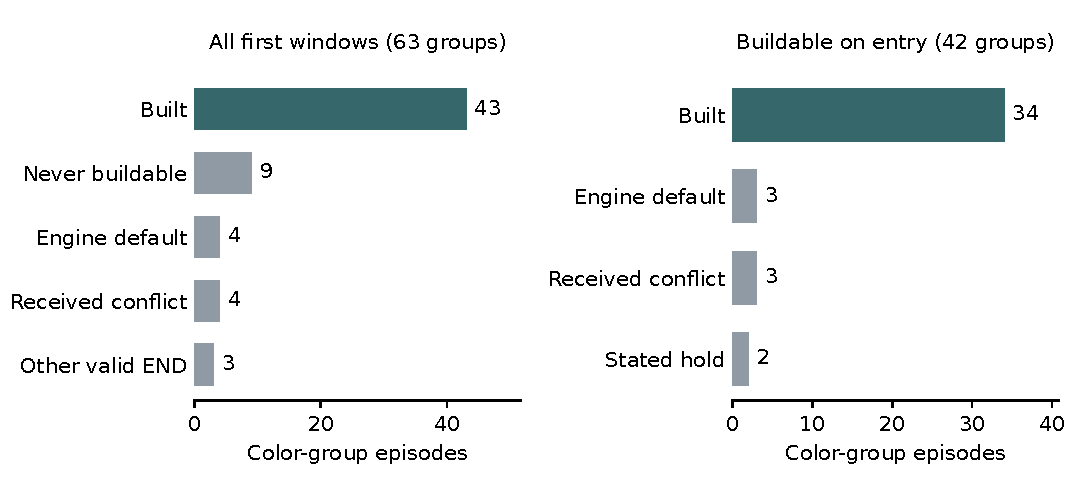
\includegraphics[width=\linewidth]{execution.pdf}
\caption{Construction after trade completion. All 63 groups have a first management window. The entry-buildable subset contains 42 groups. The two denominators describe access at different times; the received-conflict category does not assert that every content plan was executable. Source: retained first-management and residual ledgers.}
\label{fig:execution}
\end{figure}

Across all management decisions whose menu lists construction, 663 applied actions are END. Sixty-six are engine defaults, twenty-four are received calls conflicting with a named content action, and 573 have no detected name conflict. The last category includes empty or unparseable content, not 573 verified reserve choices. In particular, sixty-one of Opus's 104 ENDs in this population are defaults. Sol and Gemini's selected content fields are empty, limiting comparisons of detectable name conflicts.

\subsection{Reachable allocations fail at the action interface}

Every one of the sixty-one defaulted Opus construction purchase multisets executes at its historical state after splitting count-valued entries and ordering purchases legally. The original plans remain invalid as encoded. Sixty decisions follow a refusal with an invalid action-only response; the exceptional G2 d129 has an invalid attempt followed by a refusal. The budget is exhausted and the engine applies END. The result is a concrete failure to execute a requested investment, not evidence that the participant preferred to keep the cash.

The full construction-default population contains sixty-six decisions and seventy well-formed submitted targets, plus a malformed target and attempts with no parseable target. Sixty-three well-formed targets are reachable after reordering; seven exceed current cash. At decision level, sixty-three defaults contain at least one reachable target. All sixty-six allow some legal construction, a weaker claim. Fifty-five defaults occur in G5 and G13, and repeated allocations limit the diversity of the examples. The mechanism is well documented within this population, but it is not sixty-six independent demonstrations of a general planning defect.

Successful correction also has more than one endpoint. Among uneven-build rejections ending in construction, the initial purchase multiset is preserved in 20/25 Sol, 6/18 Gemini and 5/5 Grok decisions. Counting all uneven-rejection decisions gives 20/29, 6/19, 5/5 and 0/61 for Sol, Gemini, Grok and Opus respectively. A different legal allocation is successful execution but not exact plan preservation. G14 d145--148 eventually reaches its initial eight-house target across several management decisions in one turn. Its first correction alone does not preserve the original target.

There are genuine reserve choices as well. At G3 d176, Opus selects a valid action-only END with \$204 and states a preference for reserves over a legal \$150 house. At G1 d426, Grok consistently declines another yellow house with \$488 cash. A checked extra Atlantic purchase would reduce later liquidation capacity by the \$75 purchase-to-resale loss. These examples give economic content to restraint without claiming that restraint was optimal. They also show why the refusal-recovery condition does not make every subsequent END engine-authored.

\subsection{Current-debt finance and the hotel lock}

Fifty-six of sixty eliminations have a current debt above the generous own-asset bound in Equation~\ref{eq:bound}. These debts cannot be paid by the allowed sales and mortgages. Of the remaining four, three have legal payment sequences and one has sufficient nominal assets but inaccessible finance. This resolves the historical current-debt question; it does not decide whether earlier purchases, trades or reserve choices were wise.

The three payable cases have different mechanisms. Sol's G12 d190 and Gemini's G17 d234 accounts omit collateral unlocked by building sales. In G12 d249, Grok's content requests a sale and its attached note opposes bankruptcy, but its received call declares bankruptcy. Five legal house sales pay the \$250 debt from \$43 cash and leave \$43. That case is not a uniform failure to notice mortgages and does not demonstrate deliberate surrender. Section~\ref{sec:conduct} retains its contradictory channels.

The locked case is G7 d339. Opus holds \$390 and a clear Oriental mortgage worth \$50. Its pinks have four houses, four houses and a hotel, while the bank has no houses. The hotel cannot be downgraded, and even-selling prevents removing a lower sibling's house. The only financing move mortgages Oriental, producing \$440 and automatic bankruptcy against \$750 owed. Nominal resources total \$1,310, but the additional value is not accessible at that decision. Earlier opportunities to release houses concern different historical prefixes; they are not available debt-phase actions.

Successful and unsuccessful actual liquidations provide contrasts. G20 d327--336 combines \$700 building salvage and \$665 mortgages with \$49 cash, pays \$1,400 and retains \$14. G16's extensive liquidation instead reaches \$1,393 against \$2,000. The model's original account already has the correct total, while an early researcher label omitted unlocked collateral. These cases prevent a narrative in which every eliminated player failed to finance or every favorable-looking alternative was overlooked by the model.

\subsection{Inheritance connects local decisions to collective outcomes}

There are 103 spending units, with \$103,450 of own construction outlay, \$93,000 in whole-game paid developed rent and \$92,550 after first own expenditure. Forty units receive zero developed rent; twenty-six of those also trigger no creditor elimination. These are distinct units from the fifty-seven built-color rent elimination triggers. Zero receipts do not establish a bad investment: available exposure, unpaid final rent, inherited development and salvage differ.

Eventual winners hold fifty-eight spending units. Thirty-four contain an inherited deed at first own spending; only thirty first become complete through an estate. Four mixed-route groups contain inherited deeds but finish through a later purchase or trade. This distinction shows how inheritance can contribute to productive holdings without being their immediate completion route.

Collective cash and deed flows should also remain separate. Actual trades transfer \$28,425 through 107 directed cash flows and 207 deeds. Paid rent totals \$121,154 over 905 events. Player-creditors receive 397 inherited deeds, of which eventual winners receive 372. Removing terminal estates still leaves winners receiving 202 of 227 inherited deeds and \$7,148 of \$7,843 estate cash. The eventual winner is creditor in 35 of forty nonterminal eliminations and 54 of sixty overall. These observations describe concentration under the intact-building inheritance rule. Conditioning on the eventual winner cannot identify how much inheritance caused winning.

Two winners, Sol in G14 and Gemini in G15, never settle a trade. G15 is especially informative. Gemini completes oranges through a Tennessee purchase, builds in turn 47 and later collects \$3,250 in developed orange rent. Oranges trigger the first two eliminations, and inherited browns the last. Greens enter only through the final estate, so an earlier description attributing the win to green development was wrong. This is an observed acquisition-to-income-to-inheritance trajectory, not evidence that avoiding trades is a superior policy.

\subsection{Maintaining and revising plans}

The fixed 240-decision sample contains fifty-nine forward-looking own-action passages, thirty-six prospective opponent-capacity or outcome passages and twenty-five correction or feedback references, with overlap. A single LLM-assisted coding pass identifies these categories; fifty-three private fields are absent, all for Opus. Statements with unspecified contingencies or horizons cannot be scored as commitments. Of eight explicit named-property landing policies, six have no later matching purchase opportunity. One is fulfilled; another, G16 d103's Virginia purchase rule, meets an affordable buy menu at d159 but resolves to an auction despite a note still favoring purchase. No plan-adherence rate is inferred from these eight selected records.

Longer realized targets exist. Sol's G9 dark-blue plan at d64 reaches three houses on each deed at d163, spanning turns 29--60. G20's plan to mortgage Vermont first detours through a sale offer, then reaches the financing endpoint after rejection. Auction ceilings can also be revised or exceeded. These are observable temporal behaviors, but changed opportunities and response conflicts prevent treating every revision as learning or every divergence as forgetting.

The full recurrence ledger follows 114 uneven-construction error decisions to 109 later submitted builds, with sixty-three repetitions. Fifty-four error decisions receive a later same-decision request containing the validator error; fifty have a next submitted build, and nine repeat it. Fifty-four of all sixty-three repetitions belong to Opus, whose refusal path usually consumed the corrective opportunity. States, allocations and feedback exposure differ, and some successors occur within the same turn. The record therefore documents repair and recurrence under unequal conditions rather than estimating a causal feedback benefit or durable learning.
